\documentclass[1p]{elsarticle_modified}
%\bibliographystyle{elsarticle-num}

%\usepackage[colorlinks]{hyperref}
%\usepackage{abbrmath_seonhwa} %\Abb, \Ascr, \Acal ,\Abf, \Afrak
\usepackage{amsfonts}
\usepackage{amssymb}
\usepackage{amsmath}
\usepackage{amsthm}
\usepackage{scalefnt}
\usepackage{amsbsy}
\usepackage{kotex}
\usepackage{caption}
\usepackage{subfig}
\usepackage{color}
\usepackage{graphicx}
\usepackage{xcolor} %% white, black, red, green, blue, cyan, magenta, yellow
\usepackage{float}
\usepackage{setspace}
\usepackage{hyperref}

\usepackage{tikz}
\usetikzlibrary{arrows}

\usepackage{multirow}
\usepackage{array} % fixed length table
\usepackage{hhline}

%%%%%%%%%%%%%%%%%%%%%
\makeatletter
\renewcommand*\env@matrix[1][\arraystretch]{%
	\edef\arraystretch{#1}%
	\hskip -\arraycolsep
	\let\@ifnextchar\new@ifnextchar
	\array{*\c@MaxMatrixCols c}}
\makeatother %https://tex.stackexchange.com/questions/14071/how-can-i-increase-the-line-spacing-in-a-matrix
%%%%%%%%%%%%%%%

\usepackage[normalem]{ulem}

\newcommand{\msout}[1]{\ifmmode\text{\sout{\ensuremath{#1}}}\else\sout{#1}\fi}
%SOURCE: \msout is \stkout macro in https://tex.stackexchange.com/questions/20609/strikeout-in-math-mode

\newcommand{\cancel}[1]{
	\ifmmode
	{\color{red}\msout{#1}}
	\else
	{\color{red}\sout{#1}}
	\fi
}

\newcommand{\add}[1]{
	{\color{blue}\uwave{#1}}
}

\newcommand{\replace}[2]{
	\ifmmode
	{\color{red}\msout{#1}}{\color{blue}\uwave{#2}}
	\else
	{\color{red}\sout{#1}}{\color{blue}\uwave{#2}}
	\fi
}

\newcommand{\Sol}{\mathcal{S}} %segment
\newcommand{\D}{D} %diagram
\newcommand{\A}{\mathcal{A}} %arc


%%%%%%%%%%%%%%%%%%%%%%%%%%%%%5 test

\def\sl{\operatorname{\textup{SL}}(2,\Cbb)}
\def\psl{\operatorname{\textup{PSL}}(2,\Cbb)}
\def\quan{\mkern 1mu \triangleright \mkern 1mu}

\theoremstyle{definition}
\newtheorem{thm}{Theorem}[section]
\newtheorem{prop}[thm]{Proposition}
\newtheorem{lem}[thm]{Lemma}
\newtheorem{ques}[thm]{Question}
\newtheorem{cor}[thm]{Corollary}
\newtheorem{defn}[thm]{Definition}
\newtheorem{exam}[thm]{Example}
\newtheorem{rmk}[thm]{Remark}
\newtheorem{alg}[thm]{Algorithm}

\newcommand{\I}{\sqrt{-1}}
\begin{document}

%\begin{frontmatter}
%
%\title{Boundary parabolic representations of knots up to 8 crossings}
%
%%% Group authors per affiliation:
%\author{Yunhi Cho} 
%\address{Department of Mathematics, University of Seoul, Seoul, Korea}
%\ead{yhcho@uos.ac.kr}
%
%
%\author{Seonhwa Kim} %\fnref{s_kim}}
%\address{Center for Geometry and Physics, Institute for Basic Science, Pohang, 37673, Korea}
%\ead{ryeona17@ibs.re.kr}
%
%\author{Hyuk Kim}
%\address{Department of Mathematical Sciences, Seoul National University, Seoul 08826, Korea}
%\ead{hyukkim@snu.ac.kr}
%
%\author{Seokbeom Yoon}
%\address{Department of Mathematical Sciences, Seoul National University, Seoul, 08826,  Korea}
%\ead{sbyoon15@snu.ac.kr}
%
%\begin{abstract}
%We find all boundary parabolic representation of knots up to 8 crossings.
%
%\end{abstract}
%\begin{keyword}
%    \MSC[2010] 57M25 
%\end{keyword}
%
%\end{frontmatter}

%\linenumbers
%\tableofcontents
%
\newcommand\colored[1]{\textcolor{white}{\rule[-0.35ex]{0.8em}{1.4ex}}\kern-0.8em\color{red} #1}%
%\newcommand\colored[1]{\textcolor{white}{ #1}\kern-2.17ex	\textcolor{white}{ #1}\kern-1.81ex	\textcolor{white}{ #1}\kern-2.15ex\color{red}#1	}

{\Large $\underline{12a_{1218}~(K12a_{1218})}$}

\setlength{\tabcolsep}{10pt}
\renewcommand{\arraystretch}{1.6}
\vspace{1cm}\begin{tabular}{m{100pt}>{\centering\arraybackslash}m{274pt}}
\multirow{5}{120pt}{
	\centering
	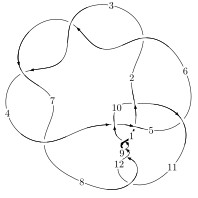
\includegraphics[width=112pt]{../../../GIT/diagram.site/Diagrams/png/2019_12a_1218.png}\\
\ \ \ A knot diagram\footnotemark}&
\allowdisplaybreaks
\textbf{Linearized knot diagam} \\
\cline{2-2}
 &
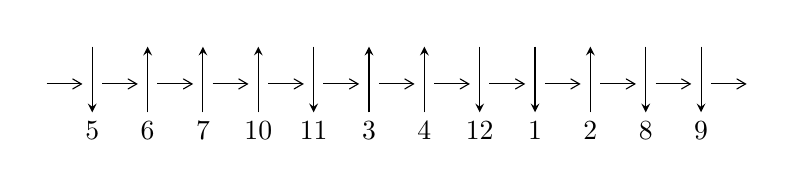
\begin{tikzpicture}[x=20pt, y=17pt]
	% nodes
	\node (C0) at (0, 0) {};
	\node (C1) at (1, 0) {};
	\node (C1U) at (1, +1) {};
	\node (C1D) at (1, -1) {5};

	\node (C2) at (2, 0) {};
	\node (C2U) at (2, +1) {};
	\node (C2D) at (2, -1) {6};

	\node (C3) at (3, 0) {};
	\node (C3U) at (3, +1) {};
	\node (C3D) at (3, -1) {7};

	\node (C4) at (4, 0) {};
	\node (C4U) at (4, +1) {};
	\node (C4D) at (4, -1) {10};

	\node (C5) at (5, 0) {};
	\node (C5U) at (5, +1) {};
	\node (C5D) at (5, -1) {11};

	\node (C6) at (6, 0) {};
	\node (C6U) at (6, +1) {};
	\node (C6D) at (6, -1) {3};

	\node (C7) at (7, 0) {};
	\node (C7U) at (7, +1) {};
	\node (C7D) at (7, -1) {4};

	\node (C8) at (8, 0) {};
	\node (C8U) at (8, +1) {};
	\node (C8D) at (8, -1) {12};

	\node (C9) at (9, 0) {};
	\node (C9U) at (9, +1) {};
	\node (C9D) at (9, -1) {1};

	\node (C10) at (10, 0) {};
	\node (C10U) at (10, +1) {};
	\node (C10D) at (10, -1) {2};

	\node (C11) at (11, 0) {};
	\node (C11U) at (11, +1) {};
	\node (C11D) at (11, -1) {8};

	\node (C12) at (12, 0) {};
	\node (C12U) at (12, +1) {};
	\node (C12D) at (12, -1) {9};
	\node (C13) at (13, 0) {};

	% arrows
	\draw[->,>={angle 60}]
	(C0) edge (C1) (C1) edge (C2) (C2) edge (C3) (C3) edge (C4) (C4) edge (C5) (C5) edge (C6) (C6) edge (C7) (C7) edge (C8) (C8) edge (C9) (C9) edge (C10) (C10) edge (C11) (C11) edge (C12) (C12) edge (C13) ;	\draw[->,>=stealth]
	(C1U) edge (C1D) (C2D) edge (C2U) (C3D) edge (C3U) (C4D) edge (C4U) (C5U) edge (C5D) (C6D) edge (C6U) (C7D) edge (C7U) (C8U) edge (C8D) (C9U) edge (C9D) (C10D) edge (C10U) (C11U) edge (C11D) (C12U) edge (C12D) ;
	\end{tikzpicture} \\
\hhline{~~} \\& 
\textbf{Solving Sequence} \\ \cline{2-2} 
 &
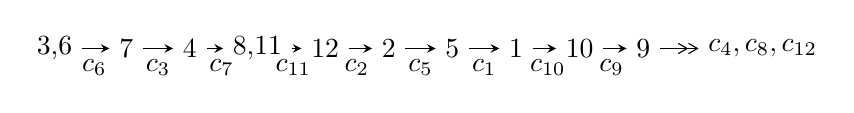
\begin{tikzpicture}[x=23pt, y=7pt]
	% node
	\node (A0) at (-1/8, 0) {3,6};
	\node (A1) at (1, 0) {7};
	\node (A2) at (2, 0) {4};
	\node (A3) at (49/16, 0) {8,11};
	\node (A4) at (33/8, 0) {12};
	\node (A5) at (41/8, 0) {2};
	\node (A6) at (49/8, 0) {5};
	\node (A7) at (57/8, 0) {1};
	\node (A8) at (65/8, 0) {10};
	\node (A9) at (73/8, 0) {9};
	\node (C1) at (1/2, -1) {$c_{6}$};
	\node (C2) at (3/2, -1) {$c_{3}$};
	\node (C3) at (5/2, -1) {$c_{7}$};
	\node (C4) at (29/8, -1) {$c_{11}$};
	\node (C5) at (37/8, -1) {$c_{2}$};
	\node (C6) at (45/8, -1) {$c_{5}$};
	\node (C7) at (53/8, -1) {$c_{1}$};
	\node (C8) at (61/8, -1) {$c_{10}$};
	\node (C9) at (69/8, -1) {$c_{9}$};
	\node (A10) at (11, 0) {$c_{4},c_{8},c_{12}$};

	% edge
	\draw[->,>=stealth]	
	(A0) edge (A1) (A1) edge (A2) (A2) edge (A3) (A3) edge (A4) (A4) edge (A5) (A5) edge (A6) (A6) edge (A7) (A7) edge (A8) (A8) edge (A9) ;
	\draw[->>,>={angle 60}]	
	(A9) edge (A10);
\end{tikzpicture} \\ 

\end{tabular} \\

\footnotetext{
The image of knot diagram is generated by the software ``\textbf{Draw programme}" developed by Andrew Bartholomew(\url{http://www.layer8.co.uk/maths/draw/index.htm\#Running-draw}), where we modified some parts for our purpose(\url{https://github.com/CATsTAILs/LinksPainter}).
}\phantom \\ \newline 
\centering \textbf{Ideals for irreducible components\footnotemark of $X_{\text{par}}$} 
 
\begin{align*}
I^u_{1}&=\langle 
-2.88764\times10^{38} u^{57}+1.08762\times10^{39} u^{56}+\cdots+1.25794\times10^{38} b+4.48859\times10^{38},\\
\phantom{I^u_{1}}&\phantom{= \langle  }-2.38160\times10^{37} u^{57}-3.45850\times10^{38} u^{56}+\cdots+1.25794\times10^{38} a-1.21766\times10^{39},\\
\phantom{I^u_{1}}&\phantom{= \langle  }u^{58}-4 u^{57}+\cdots+10 u+1\rangle \\
I^u_{2}&=\langle 
b- u,\;a-1,\;u^2+u-1\rangle \\
I^u_{3}&=\langle 
b+a,\;a^2+a-1,\;u-1\rangle \\
\\
\end{align*}
\raggedright * 3 irreducible components of $\dim_{\mathbb{C}}=0$, with total 62 representations.\\
\footnotetext{All coefficients of polynomials are rational numbers. But the coefficients are sometimes approximated in decimal forms when there is not enough margin.}
\newpage
\renewcommand{\arraystretch}{1}
\centering \section*{I. $I^u_{1}= \langle -2.89\times10^{38} u^{57}+1.09\times10^{39} u^{56}+\cdots+1.26\times10^{38} b+4.49\times10^{38},\;-2.38\times10^{37} u^{57}-3.46\times10^{38} u^{56}+\cdots+1.26\times10^{38} a-1.22\times10^{39},\;u^{58}-4 u^{57}+\cdots+10 u+1 \rangle$}
\flushleft \textbf{(i) Arc colorings}\\
\begin{tabular}{m{7pt} m{180pt} m{7pt} m{180pt} }
\flushright $a_{3}=$&$\begin{pmatrix}0\\u\end{pmatrix}$ \\
\flushright $a_{6}=$&$\begin{pmatrix}1\\0\end{pmatrix}$ \\
\flushright $a_{7}=$&$\begin{pmatrix}1\\- u^2\end{pmatrix}$ \\
\flushright $a_{4}=$&$\begin{pmatrix}u\\- u^3+u\end{pmatrix}$ \\
\flushright $a_{8}=$&$\begin{pmatrix}- u^2+1\\u^4-2 u^2\end{pmatrix}$ \\
\flushright $a_{11}=$&$\begin{pmatrix}0.189325 u^{57}+2.74933 u^{56}+\cdots+51.6861 u+9.67976\\2.29553 u^{57}-8.64604 u^{56}+\cdots-52.0009 u-3.56820\end{pmatrix}$ \\
\flushright $a_{12}=$&$\begin{pmatrix}-3.31034 u^{57}+11.1720 u^{56}+\cdots+74.9248 u+11.0418\\5.11921 u^{57}-15.5570 u^{56}+\cdots-75.3805 u-5.77324\end{pmatrix}$ \\
\flushright $a_{2}=$&$\begin{pmatrix}- u\\u\end{pmatrix}$ \\
\flushright $a_{5}=$&$\begin{pmatrix}1.35642 u^{57}-2.73919 u^{56}+\cdots-31.4858 u-5.53784\\-3.83315 u^{57}+10.5013 u^{56}+\cdots+40.7130 u+3.05633\end{pmatrix}$ \\
\flushright $a_{1}=$&$\begin{pmatrix}-1.73986 u^{57}+2.87590 u^{56}+\cdots-2.41112 u-0.766687\\1.73986 u^{57}-2.87590 u^{56}+\cdots+2.41112 u-0.233313\end{pmatrix}$ \\
\flushright $a_{10}=$&$\begin{pmatrix}-5.92742 u^{57}+17.2187 u^{56}+\cdots+94.5982 u+13.7225\\8.41228 u^{57}-23.1154 u^{56}+\cdots-94.9130 u-7.61093\end{pmatrix}$ \\
\flushright $a_{9}=$&$\begin{pmatrix}0.212480 u^{57}+0.0136304 u^{56}+\cdots+18.3659 u+6.33053\\1.59639 u^{57}-4.39858 u^{56}+\cdots-18.8215 u-1.06192\end{pmatrix}$\\&\end{tabular}
\flushleft \textbf{(ii) Obstruction class $= -1$}\\~\\
\flushleft \textbf{(iii) Cusp Shapes $= 21.4511 u^{57}-79.0212 u^{56}+\cdots-524.981 u-52.4582$}\\~\\
\newpage\renewcommand{\arraystretch}{1}
\flushleft \textbf{(iv) u-Polynomials at the component}\newline \\
\begin{tabular}{m{50pt}|m{274pt}}
Crossings & \hspace{64pt}u-Polynomials at each crossing \\
\hline $$\begin{aligned}c_{1}\end{aligned}$$&$\begin{aligned}
&u^{58}+3 u^{57}+\cdots+4 u+4
\end{aligned}$\\
\hline $$\begin{aligned}c_{2},c_{3},c_{6}\\c_{7}\end{aligned}$$&$\begin{aligned}
&u^{58}-4 u^{57}+\cdots+10 u+1
\end{aligned}$\\
\hline $$\begin{aligned}c_{4}\end{aligned}$$&$\begin{aligned}
&u^{58}- u^{57}+\cdots+519 u+83
\end{aligned}$\\
\hline $$\begin{aligned}c_{5}\end{aligned}$$&$\begin{aligned}
&u^{58}+u^{57}+\cdots-519 u+83
\end{aligned}$\\
\hline $$\begin{aligned}c_{8},c_{9},c_{11}\\c_{12}\end{aligned}$$&$\begin{aligned}
&u^{58}+4 u^{57}+\cdots-10 u+1
\end{aligned}$\\
\hline $$\begin{aligned}c_{10}\end{aligned}$$&$\begin{aligned}
&u^{58}-3 u^{57}+\cdots-4 u+4
\end{aligned}$\\
\hline
\end{tabular}\\~\\
\newpage\renewcommand{\arraystretch}{1}
\flushleft \textbf{(v) Riley Polynomials at the component}\newline \\
\begin{tabular}{m{50pt}|m{274pt}}
Crossings & \hspace{64pt}Riley Polynomials at each crossing \\
\hline $$\begin{aligned}c_{1},c_{10}\end{aligned}$$&$\begin{aligned}
&y^{58}-17 y^{57}+\cdots-120 y+16
\end{aligned}$\\
\hline $$\begin{aligned}c_{2},c_{3},c_{6}\\c_{7},c_{8},c_{9}\\c_{11},c_{12}\end{aligned}$$&$\begin{aligned}
&y^{58}-68 y^{57}+\cdots-90 y+1
\end{aligned}$\\
\hline $$\begin{aligned}c_{4},c_{5}\end{aligned}$$&$\begin{aligned}
&y^{58}+51 y^{57}+\cdots-36463 y+6889
\end{aligned}$\\
\hline
\end{tabular}\\~\\
\newpage\flushleft \textbf{(vi) Complex Volumes and Cusp Shapes}
$$\begin{array}{c|c|c}  
\text{Solutions to }I^u_{1}& \I (\text{vol} + \sqrt{-1}CS) & \text{Cusp shape}\\
 \hline 
\begin{aligned}
u &= -0.803979 + 0.621852 I \\
a &= -0.271991 + 1.151380 I \\
b &= -1.08545 - 1.13142 I\end{aligned}
 & -8.28668 - 10.95660 I & \phantom{-0.000000 } 0 \\ \hline\begin{aligned}
u &= -0.803979 - 0.621852 I \\
a &= -0.271991 - 1.151380 I \\
b &= -1.08545 + 1.13142 I\end{aligned}
 & -8.28668 + 10.95660 I & \phantom{-0.000000 } 0 \\ \hline\begin{aligned}
u &= -0.793217 + 0.521649 I \\
a &= \phantom{-}0.498912 - 1.122630 I \\
b &= \phantom{-}0.946234 + 1.016640 I\end{aligned}
 & \phantom{-0.000000 } -8.39682 I & \phantom{-0.000000 } 0 \\ \hline\begin{aligned}
u &= -0.793217 - 0.521649 I \\
a &= \phantom{-}0.498912 + 1.122630 I \\
b &= \phantom{-}0.946234 - 1.016640 I\end{aligned}
 & \phantom{-0.000000 -}8.39682 I & \phantom{-0.000000 } 0 \\ \hline\begin{aligned}
u &= \phantom{-}0.577533 + 0.730806 I \\
a &= -0.634988 - 0.459765 I \\
b &= -0.098643 + 1.074010 I\end{aligned}
 & -5.27688 + 2.48624 I & \phantom{-0.000000 } 0 \\ \hline\begin{aligned}
u &= \phantom{-}0.577533 - 0.730806 I \\
a &= -0.634988 + 0.459765 I \\
b &= -0.098643 - 1.074010 I\end{aligned}
 & -5.27688 - 2.48624 I & \phantom{-0.000000 } 0 \\ \hline\begin{aligned}
u &= \phantom{-}1.008620 + 0.380806 I \\
a &= -0.594450 - 0.045398 I \\
b &= \phantom{-}0.149754 + 0.464822 I\end{aligned}
 & \phantom{-}1.242260 - 0.522127 I & \phantom{-0.000000 } 0 \\ \hline\begin{aligned}
u &= \phantom{-}1.008620 - 0.380806 I \\
a &= -0.594450 + 0.045398 I \\
b &= \phantom{-}0.149754 - 0.464822 I\end{aligned}
 & \phantom{-}1.242260 + 0.522127 I & \phantom{-0.000000 } 0 \\ \hline\begin{aligned}
u &= -0.749389 + 0.385619 I \\
a &= -0.849917 + 1.075030 I \\
b &= -0.781148 - 0.827305 I\end{aligned}
 & \phantom{-}2.11157 - 4.30929 I & \phantom{-}3.71388 + 6.70404 I \\ \hline\begin{aligned}
u &= -0.749389 - 0.385619 I \\
a &= -0.849917 - 1.075030 I \\
b &= -0.781148 + 0.827305 I\end{aligned}
 & \phantom{-}2.11157 + 4.30929 I & \phantom{-}3.71388 - 6.70404 I\\
 \hline 
 \end{array}$$\newpage$$\begin{array}{c|c|c}  
\text{Solutions to }I^u_{1}& \I (\text{vol} + \sqrt{-1}CS) & \text{Cusp shape}\\
 \hline 
\begin{aligned}
u &= -0.154793 + 0.824875 I \\
a &= -0.217281 - 0.442528 I \\
b &= \phantom{-}0.869009 - 0.759634 I\end{aligned}
 & -10.25510 + 6.17839 I & -4.76560 - 4.41616 I \\ \hline\begin{aligned}
u &= -0.154793 - 0.824875 I \\
a &= -0.217281 + 0.442528 I \\
b &= \phantom{-}0.869009 + 0.759634 I\end{aligned}
 & -10.25510 - 6.17839 I & -4.76560 + 4.41616 I \\ \hline\begin{aligned}
u &= \phantom{-}0.668037 + 0.496903 I \\
a &= \phantom{-}0.637455 + 0.425308 I \\
b &= \phantom{-}0.087808 - 0.841653 I\end{aligned}
 & \phantom{-}1.48873 + 1.56696 I & \phantom{-}6.38155 - 7.61387 I \\ \hline\begin{aligned}
u &= \phantom{-}0.668037 - 0.496903 I \\
a &= \phantom{-}0.637455 - 0.425308 I \\
b &= \phantom{-}0.087808 + 0.841653 I\end{aligned}
 & \phantom{-}1.48873 - 1.56696 I & \phantom{-}6.38155 + 7.61387 I \\ \hline\begin{aligned}
u &= \phantom{-}0.805056\phantom{ +0.000000I} \\
a &= \phantom{-}0.0586228\phantom{ +0.000000I} \\
b &= -0.469605\phantom{ +0.000000I}\end{aligned}
 & \phantom{-}1.37980\phantom{ +0.000000I} & \phantom{-}7.84380\phantom{ +0.000000I} \\ \hline\begin{aligned}
u &= -0.614408 + 0.433410 I \\
a &= -0.65974 - 1.92027 I \\
b &= \phantom{-}0.667344 + 0.163534 I\end{aligned}
 & -9.33906 - 4.00146 I & -4.44972 + 5.66506 I \\ \hline\begin{aligned}
u &= -0.614408 - 0.433410 I \\
a &= -0.65974 + 1.92027 I \\
b &= \phantom{-}0.667344 - 0.163534 I\end{aligned}
 & -9.33906 + 4.00146 I & -4.44972 - 5.66506 I \\ \hline\begin{aligned}
u &= \phantom{-}1.176150 + 0.494013 I \\
a &= \phantom{-}0.885445 - 0.099461 I \\
b &= -0.449248 - 0.435686 I\end{aligned}
 & -6.21754 - 1.60405 I & \phantom{-0.000000 } 0 \\ \hline\begin{aligned}
u &= \phantom{-}1.176150 - 0.494013 I \\
a &= \phantom{-}0.885445 + 0.099461 I \\
b &= -0.449248 + 0.435686 I\end{aligned}
 & -6.21754 + 1.60405 I & \phantom{-0.000000 } 0 \\ \hline\begin{aligned}
u &= -0.091748 + 0.703159 I \\
a &= -0.125386 + 0.534649 I \\
b &= -0.680727 + 0.714968 I\end{aligned}
 & -2.11157 + 4.30929 I & -3.71388 - 6.70404 I\\
 \hline 
 \end{array}$$\newpage$$\begin{array}{c|c|c}  
\text{Solutions to }I^u_{1}& \I (\text{vol} + \sqrt{-1}CS) & \text{Cusp shape}\\
 \hline 
\begin{aligned}
u &= -0.091748 - 0.703159 I \\
a &= -0.125386 - 0.534649 I \\
b &= -0.680727 - 0.714968 I\end{aligned}
 & -2.11157 - 4.30929 I & -3.71388 + 6.70404 I \\ \hline\begin{aligned}
u &= \phantom{-}0.635581 + 0.189573 I \\
a &= -0.89658 + 3.23104 I \\
b &= \phantom{-}0.93416 - 2.56648 I\end{aligned}
 & -7.67427 + 0.41875 I & -15.8309 + 7.9264 I \\ \hline\begin{aligned}
u &= \phantom{-}0.635581 - 0.189573 I \\
a &= -0.89658 - 3.23104 I \\
b &= \phantom{-}0.93416 + 2.56648 I\end{aligned}
 & -7.67427 - 0.41875 I & -15.8309 - 7.9264 I \\ \hline\begin{aligned}
u &= -0.550445 + 0.243751 I \\
a &= \phantom{-}1.52059 - 0.52439 I \\
b &= \phantom{-}0.749569 + 0.393249 I\end{aligned}
 & -1.242260 - 0.522127 I & -4.85746 + 7.66329 I \\ \hline\begin{aligned}
u &= -0.550445 - 0.243751 I \\
a &= \phantom{-}1.52059 + 0.52439 I \\
b &= \phantom{-}0.749569 - 0.393249 I\end{aligned}
 & -1.242260 + 0.522127 I & -4.85746 - 7.66329 I \\ \hline\begin{aligned}
u &= \phantom{-}0.584934 + 0.061813 I \\
a &= \phantom{-}0.15128 - 2.97701 I \\
b &= \phantom{-}0.05666 + 2.44383 I\end{aligned}
 & \phantom{-0.000000 -}0.213446 I & \phantom{-0.000000 -}0. + 27.5576 I \\ \hline\begin{aligned}
u &= \phantom{-}0.584934 - 0.061813 I \\
a &= \phantom{-}0.15128 + 2.97701 I \\
b &= \phantom{-}0.05666 - 2.44383 I\end{aligned}
 & \phantom{-0.000000 } -0.213446 I & \phantom{-0.000000 } 0. - 27.5576 I \\ \hline\begin{aligned}
u &= -0.430814 + 0.285650 I \\
a &= \phantom{-}0.09371 + 2.24652 I \\
b &= -0.371702 + 0.056513 I\end{aligned}
 & -1.48873 - 1.56696 I & -6.38155 + 7.61387 I \\ \hline\begin{aligned}
u &= -0.430814 - 0.285650 I \\
a &= \phantom{-}0.09371 - 2.24652 I \\
b &= -0.371702 - 0.056513 I\end{aligned}
 & -1.48873 + 1.56696 I & -6.38155 - 7.61387 I \\ \hline\begin{aligned}
u &= -0.250271 + 0.449093 I \\
a &= -0.567142 - 0.727486 I \\
b &= -1.268190 - 0.096887 I\end{aligned}
 & -10.37260 + 0.86444 I & -7.08102 + 2.87846 I\\
 \hline 
 \end{array}$$\newpage$$\begin{array}{c|c|c}  
\text{Solutions to }I^u_{1}& \I (\text{vol} + \sqrt{-1}CS) & \text{Cusp shape}\\
 \hline 
\begin{aligned}
u &= -0.250271 - 0.449093 I \\
a &= -0.567142 + 0.727486 I \\
b &= -1.268190 + 0.096887 I\end{aligned}
 & -10.37260 - 0.86444 I & -7.08102 - 2.87846 I \\ \hline\begin{aligned}
u &= \phantom{-}1.50011\phantom{ +0.000000I} \\
a &= -0.813827\phantom{ +0.000000I} \\
b &= \phantom{-}1.76423\phantom{ +0.000000I}\end{aligned}
 & -4.86772\phantom{ +0.000000I} & \phantom{-0.000000 } 0 \\ \hline\begin{aligned}
u &= \phantom{-}1.54778 + 0.03907 I \\
a &= -0.22281 + 1.48990 I \\
b &= \phantom{-}0.058169 - 0.419643 I\end{aligned}
 & \phantom{-}5.27688 + 2.48624 I & \phantom{-0.000000 } 0 \\ \hline\begin{aligned}
u &= \phantom{-}1.54778 - 0.03907 I \\
a &= -0.22281 - 1.48990 I \\
b &= \phantom{-}0.058169 + 0.419643 I\end{aligned}
 & \phantom{-}5.27688 - 2.48624 I & \phantom{-0.000000 } 0 \\ \hline\begin{aligned}
u &= \phantom{-}0.001775 + 0.445857 I \\
a &= \phantom{-}1.000040 - 0.710446 I \\
b &= \phantom{-}0.364686 - 0.633641 I\end{aligned}
 & \phantom{-0.000000 -}1.41091 I & \phantom{-0.000000 } 0. - 3.50261 I \\ \hline\begin{aligned}
u &= \phantom{-}0.001775 - 0.445857 I \\
a &= \phantom{-}1.000040 + 0.710446 I \\
b &= \phantom{-}0.364686 + 0.633641 I\end{aligned}
 & \phantom{-0.000000 } -1.41091 I & \phantom{-0.000000 -}0. + 3.50261 I \\ \hline\begin{aligned}
u &= \phantom{-}1.57398 + 0.11293 I \\
a &= \phantom{-}0.56491 - 1.41977 I \\
b &= -0.204122 + 0.485422 I\end{aligned}
 & -1.93678 + 5.95845 I & \phantom{-0.000000 } 0 \\ \hline\begin{aligned}
u &= \phantom{-}1.57398 - 0.11293 I \\
a &= \phantom{-}0.56491 + 1.41977 I \\
b &= -0.204122 - 0.485422 I\end{aligned}
 & -1.93678 - 5.95845 I & \phantom{-0.000000 } 0 \\ \hline\begin{aligned}
u &= \phantom{-}1.58805 + 0.06429 I \\
a &= \phantom{-}0.055690 - 1.002130 I \\
b &= -1.144500 + 0.638936 I\end{aligned}
 & \phantom{-}6.21754 + 1.60405 I & \phantom{-0.000000 } 0 \\ \hline\begin{aligned}
u &= \phantom{-}1.58805 - 0.06429 I \\
a &= \phantom{-}0.055690 + 1.002130 I \\
b &= -1.144500 - 0.638936 I\end{aligned}
 & \phantom{-}6.21754 - 1.60405 I & \phantom{-0.000000 } 0\\
 \hline 
 \end{array}$$\newpage$$\begin{array}{c|c|c}  
\text{Solutions to }I^u_{1}& \I (\text{vol} + \sqrt{-1}CS) & \text{Cusp shape}\\
 \hline 
\begin{aligned}
u &= -1.59261 + 0.05649 I \\
a &= -0.10696 + 3.02763 I \\
b &= \phantom{-}0.34217 - 2.56487 I\end{aligned}
 & \phantom{-0.000000 } -1.36403 I & \phantom{-0.000000 } 0 \\ \hline\begin{aligned}
u &= -1.59261 - 0.05649 I \\
a &= -0.10696 - 3.02763 I \\
b &= \phantom{-}0.34217 + 2.56487 I\end{aligned}
 & \phantom{-0.000000 -}1.36403 I & \phantom{-0.000000 } 0 \\ \hline\begin{aligned}
u &= -1.58253 + 0.21992 I \\
a &= \phantom{-}0.43189 - 1.53582 I \\
b &= \phantom{-}0.242359 + 1.309890 I\end{aligned}
 & \phantom{-}1.93678 - 5.95845 I & \phantom{-0.000000 } 0 \\ \hline\begin{aligned}
u &= -1.58253 - 0.21992 I \\
a &= \phantom{-}0.43189 + 1.53582 I \\
b &= \phantom{-}0.242359 - 1.309890 I\end{aligned}
 & \phantom{-}1.93678 + 5.95845 I & \phantom{-0.000000 } 0 \\ \hline\begin{aligned}
u &= -1.60277 + 0.00806 I \\
a &= \phantom{-}0.94531 - 2.97432 I \\
b &= -1.17552 + 2.67763 I\end{aligned}
 & \phantom{-}7.67427 - 0.41875 I & \phantom{-0.000000 } 0 \\ \hline\begin{aligned}
u &= -1.60277 - 0.00806 I \\
a &= \phantom{-}0.94531 + 2.97432 I \\
b &= -1.17552 - 2.67763 I\end{aligned}
 & \phantom{-}7.67427 + 0.41875 I & \phantom{-0.000000 } 0 \\ \hline\begin{aligned}
u &= -1.61745 + 0.14658 I \\
a &= -0.199604 + 1.369900 I \\
b &= -0.401208 - 1.169100 I\end{aligned}
 & \phantom{-}9.33906 - 4.00146 I & \phantom{-0.000000 } 0 \\ \hline\begin{aligned}
u &= -1.61745 - 0.14658 I \\
a &= -0.199604 - 1.369900 I \\
b &= -0.401208 + 1.169100 I\end{aligned}
 & \phantom{-}9.33906 + 4.00146 I & \phantom{-0.000000 } 0 \\ \hline\begin{aligned}
u &= \phantom{-}1.62381 + 0.10972 I \\
a &= -0.13698 + 1.52608 I \\
b &= \phantom{-}1.07956 - 1.05237 I\end{aligned}
 & \phantom{-}10.25510 + 6.17839 I & \phantom{-0.000000 } 0 \\ \hline\begin{aligned}
u &= \phantom{-}1.62381 - 0.10972 I \\
a &= -0.13698 - 1.52608 I \\
b &= \phantom{-}1.07956 + 1.05237 I\end{aligned}
 & \phantom{-}10.25510 - 6.17839 I & \phantom{-0.000000 } 0\\
 \hline 
 \end{array}$$\newpage$$\begin{array}{c|c|c}  
\text{Solutions to }I^u_{1}& \I (\text{vol} + \sqrt{-1}CS) & \text{Cusp shape}\\
 \hline 
\begin{aligned}
u &= \phantom{-}1.63751 + 0.15124 I \\
a &= \phantom{-}0.28012 - 1.77911 I \\
b &= -1.14258 + 1.30370 I\end{aligned}
 & \phantom{-}8.28668 + 10.95660 I & \phantom{-0.000000 } 0 \\ \hline\begin{aligned}
u &= \phantom{-}1.63751 - 0.15124 I \\
a &= \phantom{-}0.28012 + 1.77911 I \\
b &= -1.14258 - 1.30370 I\end{aligned}
 & \phantom{-}8.28668 - 10.95660 I & \phantom{-0.000000 } 0 \\ \hline\begin{aligned}
u &= \phantom{-}1.64399 + 0.18789 I \\
a &= -0.39793 + 1.95590 I \\
b &= \phantom{-}1.21392 - 1.48592 I\end{aligned}
 & \phantom{-0.000000 -}14.0571 I & \phantom{-0.000000 } 0 \\ \hline\begin{aligned}
u &= \phantom{-}1.64399 - 0.18789 I \\
a &= -0.39793 - 1.95590 I \\
b &= \phantom{-}1.21392 + 1.48592 I\end{aligned}
 & \phantom{-0.000000 } -14.0571 I & \phantom{-0.000000 } 0 \\ \hline\begin{aligned}
u &= -1.65526 + 0.07461 I \\
a &= -0.184098 - 0.969973 I \\
b &= \phantom{-}0.710486 + 0.840147 I\end{aligned}
 & \phantom{-}10.37260 - 0.86444 I & \phantom{-0.000000 } 0 \\ \hline\begin{aligned}
u &= -1.65526 - 0.07461 I \\
a &= -0.184098 + 0.969973 I \\
b &= \phantom{-}0.710486 - 0.840147 I\end{aligned}
 & \phantom{-}10.37260 + 0.86444 I & \phantom{-0.000000 } 0 \\ \hline\begin{aligned}
u &= -1.74741\phantom{ +0.000000I} \\
a &= -0.264052\phantom{ +0.000000I} \\
b &= -0.316899\phantom{ +0.000000I}\end{aligned}
 & \phantom{-}4.86772\phantom{ +0.000000I} & \phantom{-0.000000 } 0 \\ \hline\begin{aligned}
u &= -0.113883\phantom{ +0.000000I} \\
a &= \phantom{-}5.02027\phantom{ +0.000000I} \\
b &= \phantom{-}0.684561\phantom{ +0.000000I}\end{aligned}
 & -1.37980\phantom{ +0.000000I} & -7.84380\phantom{ +0.000000I}\\
 \hline 
 \end{array}$$\newpage\newpage\renewcommand{\arraystretch}{1}
\centering \section*{II. $I^u_{2}= \langle b- u,\;a-1,\;u^2+u-1 \rangle$}
\flushleft \textbf{(i) Arc colorings}\\
\begin{tabular}{m{7pt} m{180pt} m{7pt} m{180pt} }
\flushright $a_{3}=$&$\begin{pmatrix}0\\u\end{pmatrix}$ \\
\flushright $a_{6}=$&$\begin{pmatrix}1\\0\end{pmatrix}$ \\
\flushright $a_{7}=$&$\begin{pmatrix}1\\u-1\end{pmatrix}$ \\
\flushright $a_{4}=$&$\begin{pmatrix}u\\- u+1\end{pmatrix}$ \\
\flushright $a_{8}=$&$\begin{pmatrix}u\\- u\end{pmatrix}$ \\
\flushright $a_{11}=$&$\begin{pmatrix}1\\u\end{pmatrix}$ \\
\flushright $a_{12}=$&$\begin{pmatrix}- u+1\\2 u\end{pmatrix}$ \\
\flushright $a_{2}=$&$\begin{pmatrix}- u\\u\end{pmatrix}$ \\
\flushright $a_{5}=$&$\begin{pmatrix}- u+1\\u-1\end{pmatrix}$ \\
\flushright $a_{1}=$&$\begin{pmatrix}- u\\u\end{pmatrix}$ \\
\flushright $a_{10}=$&$\begin{pmatrix}- u+1\\2 u\end{pmatrix}$ \\
\flushright $a_{9}=$&$\begin{pmatrix}1\\u\end{pmatrix}$\\&\end{tabular}
\flushleft \textbf{(ii) Obstruction class $= 1$}\\~\\
\flushleft \textbf{(iii) Cusp Shapes $= 5$}\\~\\
\newpage\renewcommand{\arraystretch}{1}
\flushleft \textbf{(iv) u-Polynomials at the component}\newline \\
\begin{tabular}{m{50pt}|m{274pt}}
Crossings & \hspace{64pt}u-Polynomials at each crossing \\
\hline $$\begin{aligned}c_{1}\end{aligned}$$&$\begin{aligned}
&u^2
\end{aligned}$\\
\hline $$\begin{aligned}c_{2},c_{3}\end{aligned}$$&$\begin{aligned}
&u^2- u-1
\end{aligned}$\\
\hline $$\begin{aligned}c_{4},c_{5},c_{6}\\c_{7}\end{aligned}$$&$\begin{aligned}
&u^2+u-1
\end{aligned}$\\
\hline $$\begin{aligned}c_{8},c_{9},c_{10}\end{aligned}$$&$\begin{aligned}
&(u-1)^2
\end{aligned}$\\
\hline $$\begin{aligned}c_{11},c_{12}\end{aligned}$$&$\begin{aligned}
&(u+1)^2
\end{aligned}$\\
\hline
\end{tabular}\\~\\
\newpage\renewcommand{\arraystretch}{1}
\flushleft \textbf{(v) Riley Polynomials at the component}\newline \\
\begin{tabular}{m{50pt}|m{274pt}}
Crossings & \hspace{64pt}Riley Polynomials at each crossing \\
\hline $$\begin{aligned}c_{1}\end{aligned}$$&$\begin{aligned}
&y^2
\end{aligned}$\\
\hline $$\begin{aligned}c_{2},c_{3},c_{4}\\c_{5},c_{6},c_{7}\end{aligned}$$&$\begin{aligned}
&y^2-3 y+1
\end{aligned}$\\
\hline $$\begin{aligned}c_{8},c_{9},c_{10}\\c_{11},c_{12}\end{aligned}$$&$\begin{aligned}
&(y-1)^2
\end{aligned}$\\
\hline
\end{tabular}\\~\\
\newpage\flushleft \textbf{(vi) Complex Volumes and Cusp Shapes}
$$\begin{array}{c|c|c}  
\text{Solutions to }I^u_{2}& \I (\text{vol} + \sqrt{-1}CS) & \text{Cusp shape}\\
 \hline 
\begin{aligned}
u &= \phantom{-}0.618034\phantom{ +0.000000I} \\
a &= \phantom{-}1.00000\phantom{ +0.000000I} \\
b &= \phantom{-}0.618034\phantom{ +0.000000I}\end{aligned}
 & -0.657974\phantom{ +0.000000I} & \phantom{-}5.00000\phantom{ +0.000000I} \\ \hline\begin{aligned}
u &= -1.61803\phantom{ +0.000000I} \\
a &= \phantom{-}1.00000\phantom{ +0.000000I} \\
b &= -1.61803\phantom{ +0.000000I}\end{aligned}
 & \phantom{-}7.23771\phantom{ +0.000000I} & \phantom{-}5.00000\phantom{ +0.000000I}\\
 \hline 
 \end{array}$$\newpage\newpage\renewcommand{\arraystretch}{1}
\centering \section*{III. $I^u_{3}= \langle b+a,\;a^2+a-1,\;u-1 \rangle$}
\flushleft \textbf{(i) Arc colorings}\\
\begin{tabular}{m{7pt} m{180pt} m{7pt} m{180pt} }
\flushright $a_{3}=$&$\begin{pmatrix}0\\1\end{pmatrix}$ \\
\flushright $a_{6}=$&$\begin{pmatrix}1\\0\end{pmatrix}$ \\
\flushright $a_{7}=$&$\begin{pmatrix}1\\-1\end{pmatrix}$ \\
\flushright $a_{4}=$&$\begin{pmatrix}1\\0\end{pmatrix}$ \\
\flushright $a_{8}=$&$\begin{pmatrix}0\\-1\end{pmatrix}$ \\
\flushright $a_{11}=$&$\begin{pmatrix}a\\- a\end{pmatrix}$ \\
\flushright $a_{12}=$&$\begin{pmatrix}a\\0\end{pmatrix}$ \\
\flushright $a_{2}=$&$\begin{pmatrix}-1\\1\end{pmatrix}$ \\
\flushright $a_{5}=$&$\begin{pmatrix}- a+2\\a-1\end{pmatrix}$ \\
\flushright $a_{1}=$&$\begin{pmatrix}- a+1\\a\end{pmatrix}$ \\
\flushright $a_{10}=$&$\begin{pmatrix}a\\- a\end{pmatrix}$ \\
\flushright $a_{9}=$&$\begin{pmatrix}- a+1\\-1\end{pmatrix}$\\&\end{tabular}
\flushleft \textbf{(ii) Obstruction class $= 1$}\\~\\
\flushleft \textbf{(iii) Cusp Shapes $= -5$}\\~\\
\newpage\renewcommand{\arraystretch}{1}
\flushleft \textbf{(iv) u-Polynomials at the component}\newline \\
\begin{tabular}{m{50pt}|m{274pt}}
Crossings & \hspace{64pt}u-Polynomials at each crossing \\
\hline $$\begin{aligned}c_{1},c_{2},c_{3}\end{aligned}$$&$\begin{aligned}
&(u+1)^2
\end{aligned}$\\
\hline $$\begin{aligned}c_{4},c_{5},c_{11}\\c_{12}\end{aligned}$$&$\begin{aligned}
&u^2- u-1
\end{aligned}$\\
\hline $$\begin{aligned}c_{6},c_{7}\end{aligned}$$&$\begin{aligned}
&(u-1)^2
\end{aligned}$\\
\hline $$\begin{aligned}c_{8},c_{9}\end{aligned}$$&$\begin{aligned}
&u^2+u-1
\end{aligned}$\\
\hline $$\begin{aligned}c_{10}\end{aligned}$$&$\begin{aligned}
&u^2
\end{aligned}$\\
\hline
\end{tabular}\\~\\
\newpage\renewcommand{\arraystretch}{1}
\flushleft \textbf{(v) Riley Polynomials at the component}\newline \\
\begin{tabular}{m{50pt}|m{274pt}}
Crossings & \hspace{64pt}Riley Polynomials at each crossing \\
\hline $$\begin{aligned}c_{1},c_{2},c_{3}\\c_{6},c_{7}\end{aligned}$$&$\begin{aligned}
&(y-1)^2
\end{aligned}$\\
\hline $$\begin{aligned}c_{4},c_{5},c_{8}\\c_{9},c_{11},c_{12}\end{aligned}$$&$\begin{aligned}
&y^2-3 y+1
\end{aligned}$\\
\hline $$\begin{aligned}c_{10}\end{aligned}$$&$\begin{aligned}
&y^2
\end{aligned}$\\
\hline
\end{tabular}\\~\\
\newpage\flushleft \textbf{(vi) Complex Volumes and Cusp Shapes}
$$\begin{array}{c|c|c}  
\text{Solutions to }I^u_{3}& \I (\text{vol} + \sqrt{-1}CS) & \text{Cusp shape}\\
 \hline 
\begin{aligned}
u &= \phantom{-}1.00000\phantom{ +0.000000I} \\
a &= \phantom{-}0.618034\phantom{ +0.000000I} \\
b &= -0.618034\phantom{ +0.000000I}\end{aligned}
 & \phantom{-}0.657974\phantom{ +0.000000I} & -5.00000\phantom{ +0.000000I} \\ \hline\begin{aligned}
u &= \phantom{-}1.00000\phantom{ +0.000000I} \\
a &= -1.61803\phantom{ +0.000000I} \\
b &= \phantom{-}1.61803\phantom{ +0.000000I}\end{aligned}
 & -7.23771\phantom{ +0.000000I} & -5.00000\phantom{ +0.000000I}\\
 \hline 
 \end{array}$$\newpage
\newpage\renewcommand{\arraystretch}{1}
\centering \section*{ IV. u-Polynomials}
\begin{tabular}{m{50pt}|m{274pt}}
Crossings & \hspace{64pt}u-Polynomials at each crossing \\
\hline $$\begin{aligned}c_{1}\end{aligned}$$&$\begin{aligned}
&u^2(u+1)^2(u^{58}+3 u^{57}+\cdots+4 u+4)
\end{aligned}$\\
\hline $$\begin{aligned}c_{2},c_{3}\end{aligned}$$&$\begin{aligned}
&((u+1)^2)(u^2- u-1)(u^{58}-4 u^{57}+\cdots+10 u+1)
\end{aligned}$\\
\hline $$\begin{aligned}c_{4}\end{aligned}$$&$\begin{aligned}
&(u^2- u-1)(u^2+u-1)(u^{58}- u^{57}+\cdots+519 u+83)
\end{aligned}$\\
\hline $$\begin{aligned}c_{5}\end{aligned}$$&$\begin{aligned}
&(u^2- u-1)(u^2+u-1)(u^{58}+u^{57}+\cdots-519 u+83)
\end{aligned}$\\
\hline $$\begin{aligned}c_{6},c_{7}\end{aligned}$$&$\begin{aligned}
&((u-1)^2)(u^2+u-1)(u^{58}-4 u^{57}+\cdots+10 u+1)
\end{aligned}$\\
\hline $$\begin{aligned}c_{8},c_{9}\end{aligned}$$&$\begin{aligned}
&((u-1)^2)(u^2+u-1)(u^{58}+4 u^{57}+\cdots-10 u+1)
\end{aligned}$\\
\hline $$\begin{aligned}c_{10}\end{aligned}$$&$\begin{aligned}
&u^2(u-1)^2(u^{58}-3 u^{57}+\cdots-4 u+4)
\end{aligned}$\\
\hline $$\begin{aligned}c_{11},c_{12}\end{aligned}$$&$\begin{aligned}
&((u+1)^2)(u^2- u-1)(u^{58}+4 u^{57}+\cdots-10 u+1)
\end{aligned}$\\
\hline
\end{tabular}\newpage\renewcommand{\arraystretch}{1}
\centering \section*{ V. Riley Polynomials}
\begin{tabular}{m{50pt}|m{274pt}}
Crossings & \hspace{64pt}Riley Polynomials at each crossing \\
\hline $$\begin{aligned}c_{1},c_{10}\end{aligned}$$&$\begin{aligned}
&y^2(y-1)^2(y^{58}-17 y^{57}+\cdots-120 y+16)
\end{aligned}$\\
\hline $$\begin{aligned}c_{2},c_{3},c_{6}\\c_{7},c_{8},c_{9}\\c_{11},c_{12}\end{aligned}$$&$\begin{aligned}
&((y-1)^2)(y^2-3 y+1)(y^{58}-68 y^{57}+\cdots-90 y+1)
\end{aligned}$\\
\hline $$\begin{aligned}c_{4},c_{5}\end{aligned}$$&$\begin{aligned}
&((y^2-3 y+1)^2)(y^{58}+51 y^{57}+\cdots-36463 y+6889)
\end{aligned}$\\
\hline
\end{tabular}
\vskip 2pc
\end{document}